\documentclass[main.tex]{subfiles}

\begin{document}

\section{Aufgabe 2}
Von einer Zufallsvariablen $X$ wird vermutet, dass sie die nebenstehende Dichte $f$ besitzt mit $f(x) = 0$ für $x \neq [0; 3]$.
\begin{center}
	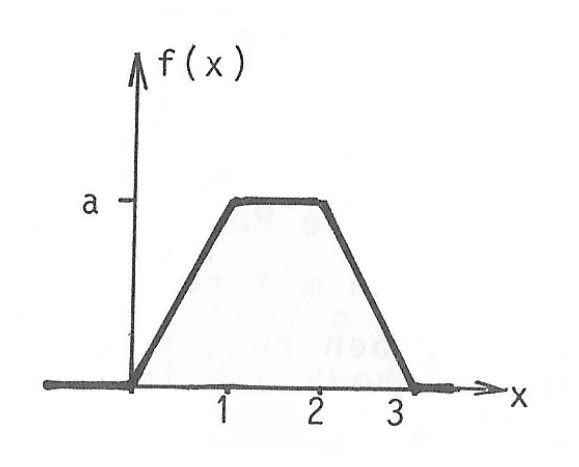
\includegraphics[scale=0.5]{Stochastik_III.4.10b_A02_Dichtefkt.jpg}
\end{center}
\begin{enumerate}
\item Bestimmen Sie die Konstante $a$ so, dass $f$ eine Dichte ist.
\item Testen Sie die Vermutung mit folgender Stichprobe zum Niveau $\alpha = 0,05$:
\begin{center}
	\begin{tabular}{c|c}
		Klasse & abs. Häufigkeit \\ \hline
		$[0; 1]$ & $15$ \\
		$(1; 2]$ & $29$ \\
		$(2; 3]$ & $6$
	\end{tabular}
\end{center}
\end{enumerate}

\subsection{Lösung 2}

\end{document}
